\documentclass[conference]{IEEEtran}
\IEEEoverridecommandlockouts
% The preceding line is only needed to identify funding in the first footnote. If that is unneeded, please comment it out.
% \usepackage{cite}
\usepackage{amsmath,amssymb,amsfonts}
\usepackage{algorithmic}
\usepackage{graphicx}
\usepackage{textcomp}
\usepackage{xcolor}
\usepackage{balance}
\usepackage{subcaption}
%\def\BibTeX{{\rm B\kern-.05em{\sc i\kern-.025em b}\kern-.08em
%    T\kern-.1667em\lower.7ex\hbox{E}\kern-.125emX}}

\usepackage[backend=biber,style=numeric,sorting=none]{biblatex} %Imports biblatex package
\addbibresource{lit.bib} %Import the bibliography file

\begin{document}
\balance

\title{Robustness Testing of Image Classifiers Using Genetic Algorithms\\{}}

\author{
\IEEEauthorblockN{Martin Hallgren\IEEEauthorrefmark{1},
Kyu-Sang Kim\IEEEauthorrefmark{2},
Fried Kullmann\IEEEauthorrefmark{3},
Thomas Mattsson\IEEEauthorrefmark{4} and
Mikkel Odgaard\IEEEauthorrefmark{5}}
\IEEEauthorblockA{\IEEEauthorrefmark{1}Linköping University, Linköping, Sweden\\
Email: marha805@student.liu.se - GitHub: Martin-Hallgren}
\IEEEauthorblockA{\IEEEauthorrefmark{2}School of Computer Science and Engineering\\
University of New South Wales, Sydney, Australia\\
Email: kyu-sang.kim@unsw.edu.au - GitHub: Choco3-3}
\IEEEauthorblockA{\IEEEauthorrefmark{3}
TU Dortmund University, Dortmund, Germany\\
Email: fried.kullmann@tu-dortmund.de - GitHub: ChristPi}
\IEEEauthorblockA{\IEEEauthorrefmark{4}Technical University of Denmark, Kongens Lyngby, Denmark \\
Email: s175206@student.dtu.dk - GitHub: Tmattsson0}
\IEEEauthorblockA{\IEEEauthorrefmark{5}Technical University of Denmark, Kongens Lyngby, Denmark \\
Email: s174371@student.dtu.dk - Github: mikkelfo}
\IEEEauthorblockA{GitHub: https://github.com/mikkelfo/CS454-Robustness-Testing-for-Neural-Networks}}

\maketitle
\begin{abstract}
Image recognition is more popular than ever before, and with so many applications whose critical components rely on the accuracy of an image classifier, there is a big interest in making image classifiers more robust.
This paper is trying to test the robustness of image classifiers by using a genetic algorithm to find the most sensitive parts of the image where added artifacts can fool it.

The methodology we follow is not about using adversarial attacks, but rather generating real-world conditions such as illumination changes and lens-scratches. This is done by applying a mask containing random shapes to images.

From our experiments, it was shown that the parameters we tuned had little to no effect on the final results.
The characteristics of the generated masks showed that if a small number of shapes were added, the shapes would tend to be around the center and be red and blue. If a mask had many shapes, a majority of these would often be green.

Our solution uses simple shapes to test the robustness of the image classifier, but in future versions of this project, other methods should be explored.
This could include having the genetic algorithm find more complex shapes or perhaps adding realistic shapes like raindrops and scratches onto the image.
\end{abstract}

\begin{IEEEkeywords}
genetic algorithms, GA, adversarial attack, robustness, search-based testing
\end{IEEEkeywords}

\section{Introduction}
Image recognition is an important technology in today's world.
It is used in everything from social media apps to self-driving cars.
With the importance of the applications and services that use this technology, there has been an incentive to keep improving it.
And with more processing power and better cameras, image recognition has become significantly better.
However, software with image recognition is known to be fragile and highly influenced by lighting changes or image noise.
This is why the robustness of these models is important.
But since training image recognition models require a large number of labeled images, it can be challenging to test the robustness of an image classification or recognition system, since it would require many variations of the same scene or object.

Therefore, there is a desire to be able to test the robustness of an image classifier without having to increase the number of images.
Other work has been done on this issue. 
One example uses an algorithm that tries to estimate the robustness of a classifier and identify "weak spots" by randomly and semi-randomly applying noise to a picture \cite{Robust_image_thesis}.
This paper concludes that classifiers are quite resilient to random noise. 
However, they can quickly fail when semi-random noise, i.e., mostly random noise but with tunable parameters, is applied.

To better find these "weak spots", we approached this problem as a \textit{search-based problem}.
Search-based techniques are quite suited for this scenario, as it is unknown how the classifier classifies every image, making it hard to make an effective general-purpose algorithm.
By using a \textit{genetic algorithm}, we can build a more general way of finding these "weak spots".

Given an image classifier and a set of labeled test images, our program first runs the classifier on the images without modification to get a baseline. 
Then it applies a mask to the images populated with various shapes that modify the RGB values of the original images. 
The images are then classified again to get a new accuracy.
This accuracy and the amount of change in the pixels are the two objectives the genetic algorithm tries to optimize.
This is repeated for several generations to keep improving the fitness of the masks being applied.
The goal of the genetic algorithm is to get the classifier to misclassify the image by changing as little as possible and expose "weaknesses". Weaknesses being certain mask or shape characteristics that the image classifier has a hard time dealing with. 


\section{Method}
We do not aim to attack the neural network with an adversarial attack, which is a carefully constructed attack that targets specific neurons to force a misclassification to a specified class.
We want to simulate real-world examples of "attacks", e.g., a scratch on a lens or a darkened area. 
We apply a \textit{mask} to the picture, which contains simulated real-life damages.
Our genetic algorithm is in charge of constructing these simulated damages.

To explain our methodology, from a bottom-up approach, we start from a \textit{point}.
A single point is simply a pixel.
A group of points, scattered randomly in a constrained area, makes up a convex-hull, which is denoted a \textit{shape}.
This means that a shape is the convex hull of these points, i.e., the maximum area contained by connecting points.
We then denote a collection of shapes as a \textit{mask}, the highest level of our hierarchy. 

A shape consists of a collection of points, as well as a center point.
The center point is randomly generated, and the other points are randomly put around it, with a maximum distance of 30 pixels.
A shape is therefore contained in a 61x61 square, centered in the center point.
Furthermore, each shape has its own attribute, its pixel change.
Each shape is set up with a list of attributes corresponding to the RGB change, from -255 to 255. 
This means that a shape with an RGB change of [-255, 0, 255] will affect its area's (the convex hull from the collection of points) red values by -255, thus capping out at 0, will not change the green values and lastly increase the blue values by 255, capping out at 255.
Lastly, we have a shape's area.
Since we are dealing with pixels, which is not defined by floats, but integers, we cannot simply calculate the area of the convex hull.
Instead, we look at the number of pixels in the area, which better represents how large a shape is. 

A mask will hold the high-level attributes, such as the amount of change, measured by the sum of each shape's area times the absolute change in RGB values. 
Applied to the images, the classifier's accuracy change gives us the second objective's fitness function.

\subsection{Crossover}

To create an offspring from two parent masks, we apply crossover on the shapes of the parents.
Since the ordering of the shapes in the mask does not matter, we pick a random number of shapes from both parents and combine them in the offspring.
The shapes themselves can only be modified by mutation.

\subsection{Mutation}

There are three different ways to mutate a shape: point-wise, shape-wise, and RGB-wise.

\begin{itemize}
\item{Changing the shape}: The shape is determined by the convex hull of a set of points, so to mutate the shape, a point can be added, removed, or moved.
\item {Moving the shape}: The shape can be shifted in any constrained distance.
\item {Changing the RGB value}: Each color value of the  RGB value change applied to the image can be altered to either a higher or lower value.
\end{itemize}

\subsection{Selection}
For the selection, we choose two random parents from the population and produce one offspring every generation.

\subsection{Generational Selection}

Every generation, one offspring is produced and compared on a Pareto-front against the existing population. 
The offspring are added to the population if the offspring is not dominated by another individual in the population.
If any individuals are dominated by the offspring, those individuals are removed from the population.

\subsection{Pareto-front}

A mask has two fitness values, the accuracy of the classifier after the mask has been applied and how much change was applied to the images, where we want to maximize the accuracy drop of the classifier and minimize the changes to the images
Since we have two objectives, we use a Pareto-front to evaluate the fitness of each individual. 

How much change is applied by a mask is measured by the sum of the change of all shapes in the mask.
A shape's change is the sum of the absolute RGB values times the number of pixels in the shape.
Thus, the change of a mask is calculated as follows:
\[
Change = \sum _{k=1}^{n}(\left |R_{k} \right|+\left |G_{k} \right|+\left |B_{k} \right|)*p_{k}
\]
Where \textit{n} is the number of shapes in the mask and $p_k$ the number of pixels in the shape $k$.

\section{Experimental Setup}

For the experiments, we used the Inception V3 image classifier \cite{inception} and 1000 pictures of the ILSVRC2012 validation dataset \cite{imagenet}.
The genetic algorithm was set up with random seeding and the methods mentioned before.
The genetic algorithm approximates the Pareto-front, which represents the tradeoff between change and accuracy.
By visualizing the masks, we want to gain insight into the behavior of the image classifiers as well as why the mask reduces the accuracy.
With this information, we then want to gain insight into the weakness or rather the robustness.
The genetic algorithm is set up this way to reduce the search space as well as making it a bit more realistic.
A secondary goal is to tune the parameters of the genetic algorithm to see which settings perform the best, as this also might give insight into the model.

\begin{figure*}[htbp]
\centering
\begin{subfigure}[t]{.4\textwidth}
  \centering
  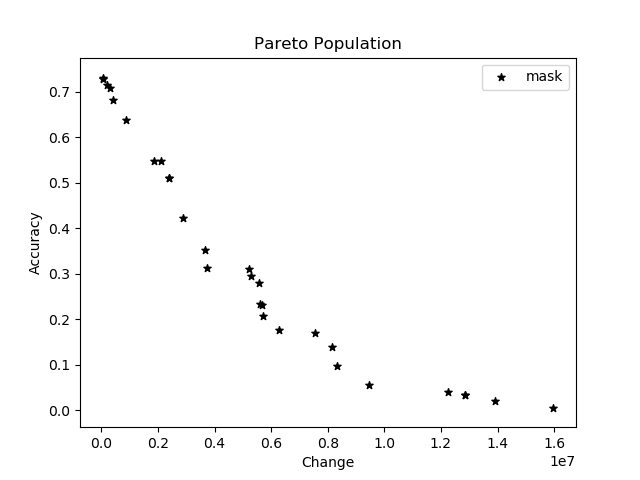
\includegraphics[width=1\linewidth]{fig/paretoplot1.png}
  \subcaption{Pareto front with maximum shapes of 30}
\end{subfigure}
\begin{subfigure}[t]{.4\textwidth}
  \centering
  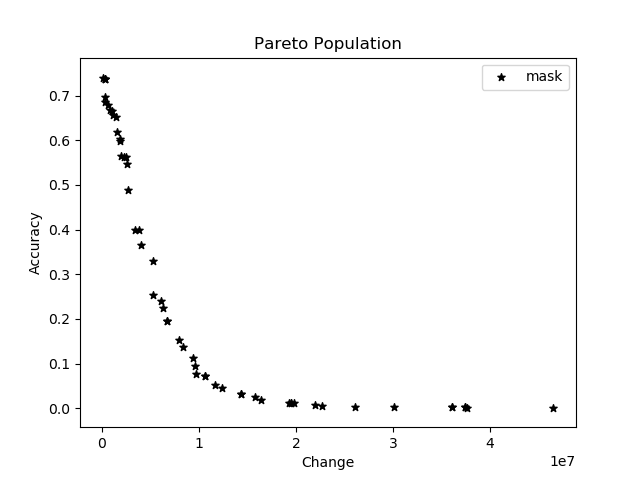
\includegraphics[width=1\linewidth]{fig/paretoplot2.png}
  \subcaption{Pareto front with maximum shapes of 40}
\end{subfigure}
\caption{Pareto fronts with different parameters. Original images from \cite{imagenet}.}
\label{fig:pareto_graphs}
\end{figure*}

\section{Results}

After tuning the parameters for the genetic algorithm, we came to the following conclusions.
The size of the starting population is mostly irrelevant as it only needs to be large enough to cover the spectrum of comparable solutions. 
Anything above that threshold hardly increased effectiveness as most of the starting population are quickly dominated and thus are not worth the computational effort.
Increasing the maximum number of shapes allowed in a mask also provided minimal benefit for the genetic algorithm as it only caused the coverage of the search space to increase, as can be seen in Figure \ref{fig:pareto_graphs}.
Although other parameters are potentially correlated to the performance of the genetic algorithm, we only observed negligible effects on the genetic algorithm unless they were more extreme.
    
\begin{figure*}[htbp]
\centering
\begin{subfigure}[t]{.4\textwidth}
  \centering
  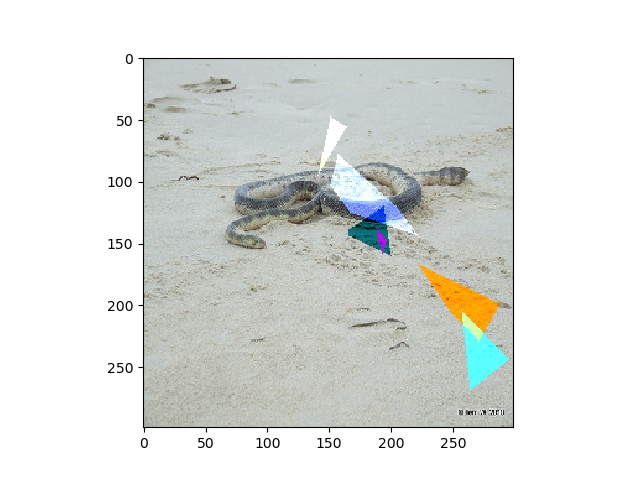
\includegraphics[width=1\linewidth]{fig/misclass1.png}
  \subcaption{Misclassification in the detail\\sea snake $\rightarrow$ sand viper}
\end{subfigure}
\begin{subfigure}[t]{.4\textwidth}
  \centering
  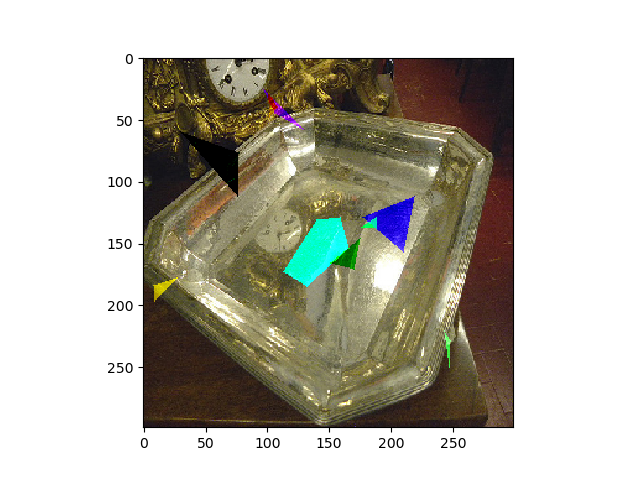
\includegraphics[width=1\linewidth]{fig/misclass2.png}
  \subcaption{Misclassification through misdireciton\\tray $\rightarrow$ analog clock}
\end{subfigure}
\\
\begin{subfigure}[t]{.4\textwidth}
  \centering
  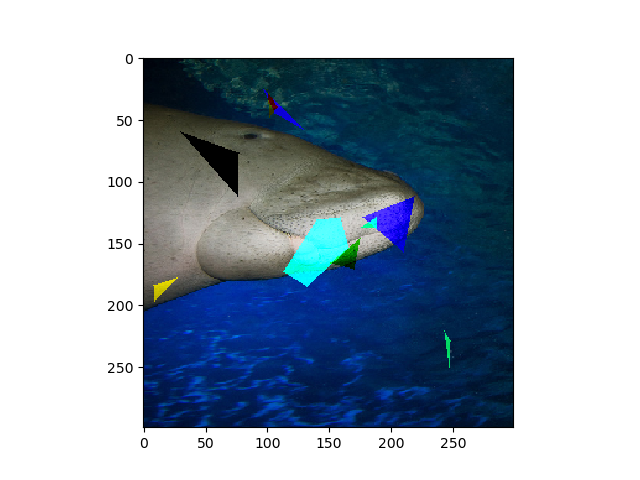
\includegraphics[width=1\linewidth]{fig/misclass3.png}
  \subcaption{Misclassification to a similar class\\dugong $\rightarrow$ white shark}
\end{subfigure}
\begin{subfigure}[t]{.4\textwidth}
  \centering
  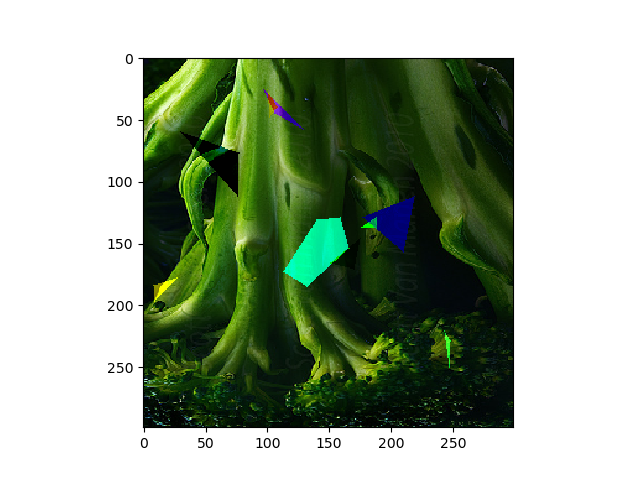
\includegraphics[width=1\linewidth]{fig/misclass4.png}
  \subcaption{Incomprehensible misclassification\\broccoli $\rightarrow$ triceratops}
\end{subfigure}
\caption{Different kinds of misclassification. Original images from \cite{imagenet}.}
\label{fig:Misclassify}
\end{figure*}

The mask characteristics were also found to be peculiar.
Masks with a low amount of shapes mostly had their shapes around the center of the image and had often more red and blue colours than green whilst masks with a high amount of shapes had many green shapes.
We can attribute this as a consequence of the narrow selection of classes and the training images which feature a disproportionately large amount of animals that include a green environment.

The misclassified images could be categorized into four different groups.
The first group consists of images that were only slightly misclassified due to the mask covering small details and thus misidentifying traits such as a dog being classified as a different breed and other similar cases.
The second group consists of images that were misclassified due to the mask covering parts of the object and thus making a different object in the image the dominant class.
The third group is similar to the first group. 
However, the images in the group are slightly misclassified to something similar but with less clarity as in the first group, such as misclassifying a cinema as a restaurant, dial phone as a sewing machine, or a dugong as a white shark.
The fourth group consists of incomprehensive classifications, where the image gets classified as something completely different and seemingly random.
Example images showcasing the different categories can be seen in Figure \ref{fig:Misclassify}.
Even though the majority of misclassifications belong to the first three groups, the images belonging to the forth are the most relevant for finding "weaknesses" in the classifier.

A special subgroup of the fourth group are classes that are "magnets" for misclassification, where images are often misclassified as "magnet" classes for no humanly logical reason.
Examples of these "magnet" classes are pinwheel, mortarboard, bandaid, and umbrella.
Example images can be seen in Figure \ref{fig:magnets}.
Some of these can be explained by the nature of the shapes and masks.

\begin{figure*}[htbp]
\centering
\begin{subfigure}{.3\textwidth}
  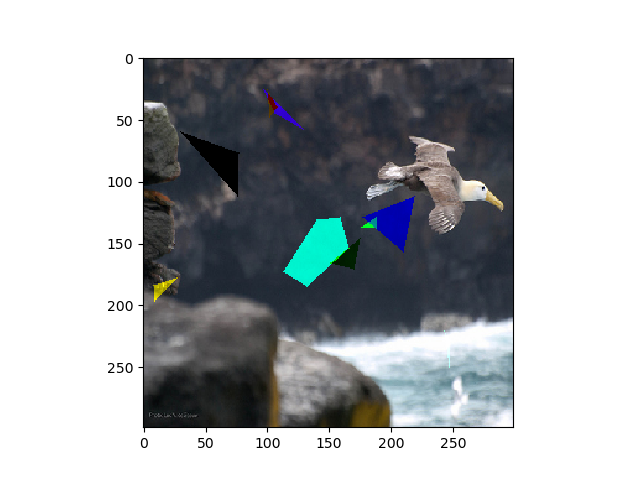
\includegraphics[width=1\linewidth]{fig/albatross-mortarboard.png}
\end{subfigure}
\begin{subfigure}{.3\textwidth}
  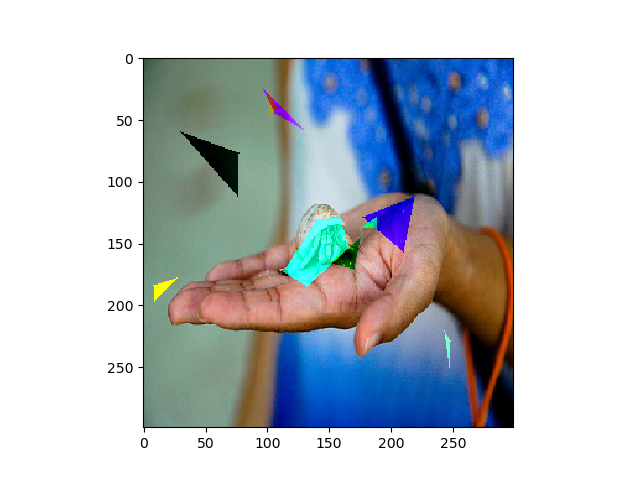
\includegraphics[width=1\linewidth]{fig/hermitcrab-motarboard.png}
\end{subfigure}
\begin{subfigure}{.3\textwidth}
  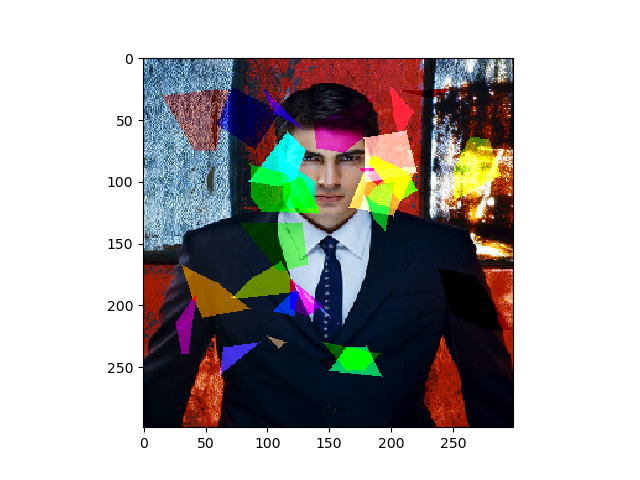
\includegraphics[width=1\linewidth]{fig/mortarboard.png}
\end{subfigure}
\begin{subfigure}[t]{.3\textwidth}
  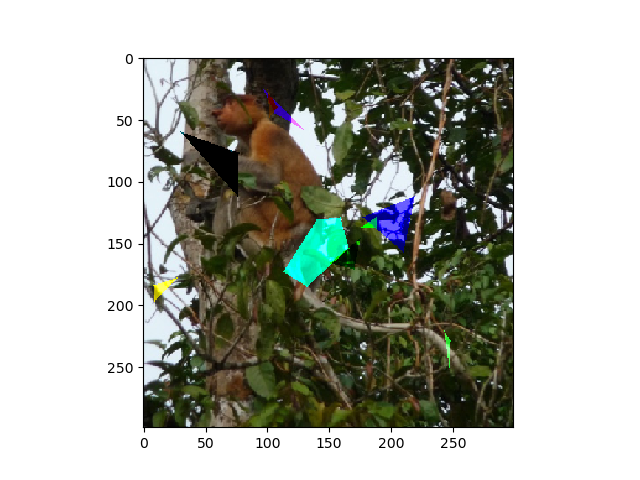
\includegraphics[width=1\linewidth]{fig/proboscismonkey-pinwheel.png}
\end{subfigure}
\begin{subfigure}[t]{.3\textwidth}
  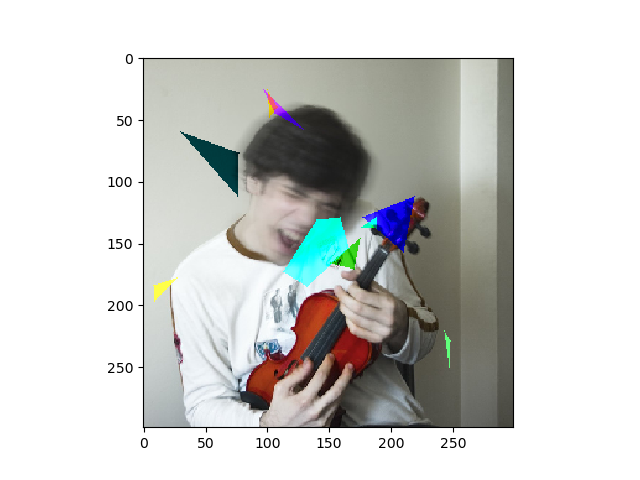
\includegraphics[width=1\linewidth]{fig/violin-pinwheel.png}
\end{subfigure}
\begin{subfigure}[t]{.3\textwidth}
  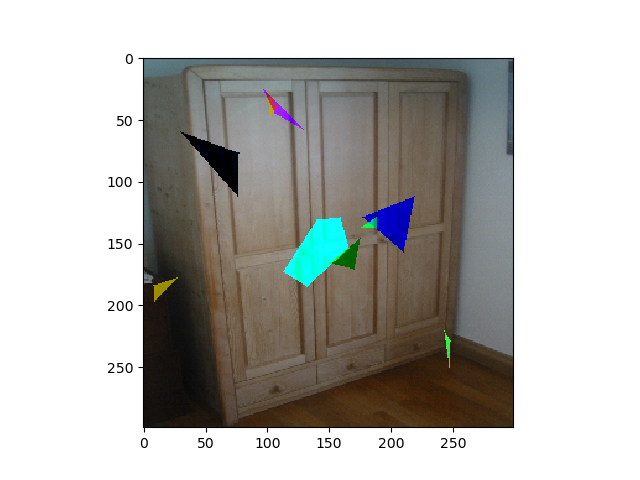
\includegraphics[width=1\linewidth]{fig/wardrobe-pinwheel.png}
\end{subfigure}
\caption{Examples for misclassification magnets. Top row: mortarboard, bottom row: pinwheel. Original images from \cite{imagenet}.}
\label{fig:magnets}
\end{figure*}

Robustness is hard to define quantitatively but some subjective general trends were observed in the Pareto-fronts and masks.
Masks with a change value above 500000 were already crowded with shapes, and images were unrecognizable with masks above one million.
That is why most images shown are all modified with masks with change values below 500000 to simulate more realistic attacks.
The mask shown in most of the images already causes an accuracy drop of 20\%.
The Pareto-fronts show that accuracy can be influenced quite heavily with small changes until it reaches about 30\%.
To decrease accuracy even further, many more shapes/changes are needed and shows a robust baseline for the classifier.
As many misclassified images are from the first three groups, these can be still acceptable and can be argued to also show the robustness of the classifier.
The images from the forth group, however, are the weaknesses of the classifier and can be used to improve the classifier.
As an example, Figure \ref{fig:ant} shows that in the ant class, the environment in the image might play too big of a role for the classification.

\begin{figure*}[htbp]
\centering
  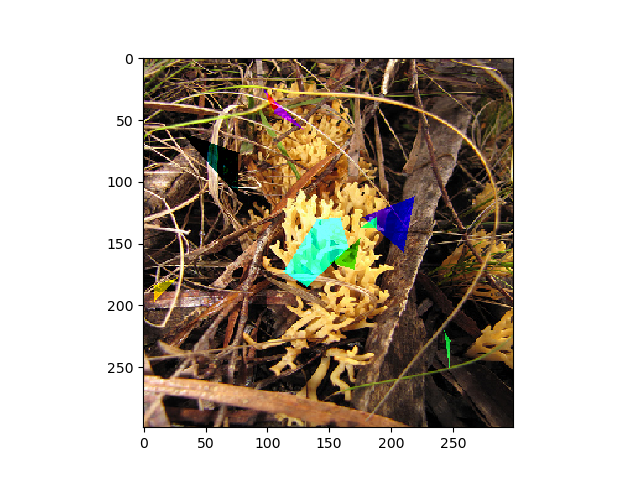
\includegraphics[width=1\linewidth]{fig/coralfungus-ant.png}
\caption{Example of group 4 misclassification indicating a weakness of the classifier}
\label{fig:ant}
\end{figure*}

\section{Threats to validity}
A threat to the generality of our results is that we have only evaluated our genetic algorithm on one classifier and on a very small subset of one dataset's validation images.

A more subtle threat is the large amount of parameters which we decided to hard-code and not subject to tuning due to the high computational cost of running and getting results of each configuration.
This includes parameters that constrained movement (such as in mutation), sizes of the shape (although some experimentation was done here) or amount of maximum points in a shape.
While these parameters are not likely to have a high impact, they might have more impact, than we give them credit for. 


\section{Discussion}
% Different characteristics of masks and our findings.
% What could have been done better
% Threats to validity
% Convex hull makes only triangles and squares.
\subsection{Representation of shapes}
We chose to make the shapes by plotting a random point along with several more points within a given limit.
These points are then used to make a convex hull.
These shapes are relatively easy to make computationally, but can never get very complex, e.g., stars or crosses.
Other ways to make shapes could maybe have been used to see what the genetic algorithm would favor, simple or complex.
However, the time complexity of drawing complex shapes that use all points was higher than convex hull.
Therefore complex shapes were not included due to the already very high computation time.

Utilising convex hulls has the potential drawback that mutation may only change the shape very little, if at all.
Due to the definition of a convex hull, all points that are not part of the shapes "border" will not, if removed, change the overall shape.
For shapes with many points, there is more likely more points "inside" the shape that there is on the edges of the shape, and so removing a point is more likely not to do anything.
This is something we need to address if we need to scale up the number of points we use to make the shape.
A worst-case scenario would be a triangle made of up 100 points, but only 3 making up the border.
A triangle like this would be very unlikely to be changed by the mutation proposed.
Going with shapes where every point is used to draw the "border", every removal would be guaranteed to change the shape. 

It is unclear how changing to complex shapes would affect our results but is something that could be tested in future work.

\subsection{Real World Use}
The reason behind doing this project was to try and find potential weaknesses in an image classifier, and by doing so, have an easier way to test different image classifiers.

From our results, it can be seen that our genetic algorithm is effective in getting the image classifier to misclassify the different images. However, when looking at the actual shapes that the genetic algorithm has put on the image, it looks like confetti.
Our program is only capable of making simple shapes that uniformly change the color, which means the “confetti-like” shapes are to be expected.
 These types of shapes do not represent a realistic scenario that any image classifier has to overcome in the real world, and so misclassification may be more common.

We can introduce realism in two ways.
First, we can try to study real-world deficits, e.g., size, shapes, colors, schemes, etc.
Some simple shapes or a grey-scale color scheme might thereby be preferred over this confetti-style.
These preferences can be either introduced via seeding or hard-coded constraints, such as 5-10 defined shapes to pick from.
Another approach, to get results that more closely match what an image classifier can be challenged by in the real world, more complex image manipulation should be thought up.
Instead of only doing simple uniformly colored shapes, it could be relevant to apply real-life obstructions such as flies, drops, cracks, and so on.
Also, changing the image illumination and the noise level could be an additional approach to the problem, as this is something image recognition systems can have hard time to deal with.
It can, however, lead to hard to identify weak spots when applying a uniform mask to an image, so experimentation with different noise and illumination intensities throughout the mask would have to be done.

It is possible that using these more realistic approaches could help show real-life weaknesses in the classifier.
It is something that, if work on this project was to continue, would be interesting to test.  

\section{Future work}
In this section, we will briefly sum up the discussion points to a more coherent approach.
As mentioned in the discussion, two different routes can be taken.
The first route will have the genetic algorithm find shapes, as done in this project, but with added constraints and domain knowledge, in order to get more real-life shapes.
The second approach will \textit{not} model shapes, but rather select from a predefined set of real-world objects, such as flies, scratches, raindrops, or cracks.
Both methods would tackle problematic considerations we had in the project, namely the shape and the color of the obstructions.
Moreover, instead of testing a single classifier, more classifiers should be tested, so that their robustness can be directly compared, thereby creating an additional evaluation metric, robustness.
In the future, it is not enough to only look at a classifier's accuracy and speed, if it is easily disrupted.

\section{References}
\printbibliography[heading=none]

\end{document}